
\documentclass[../main.tex]{subfiles}

\begin{figure}[r]
	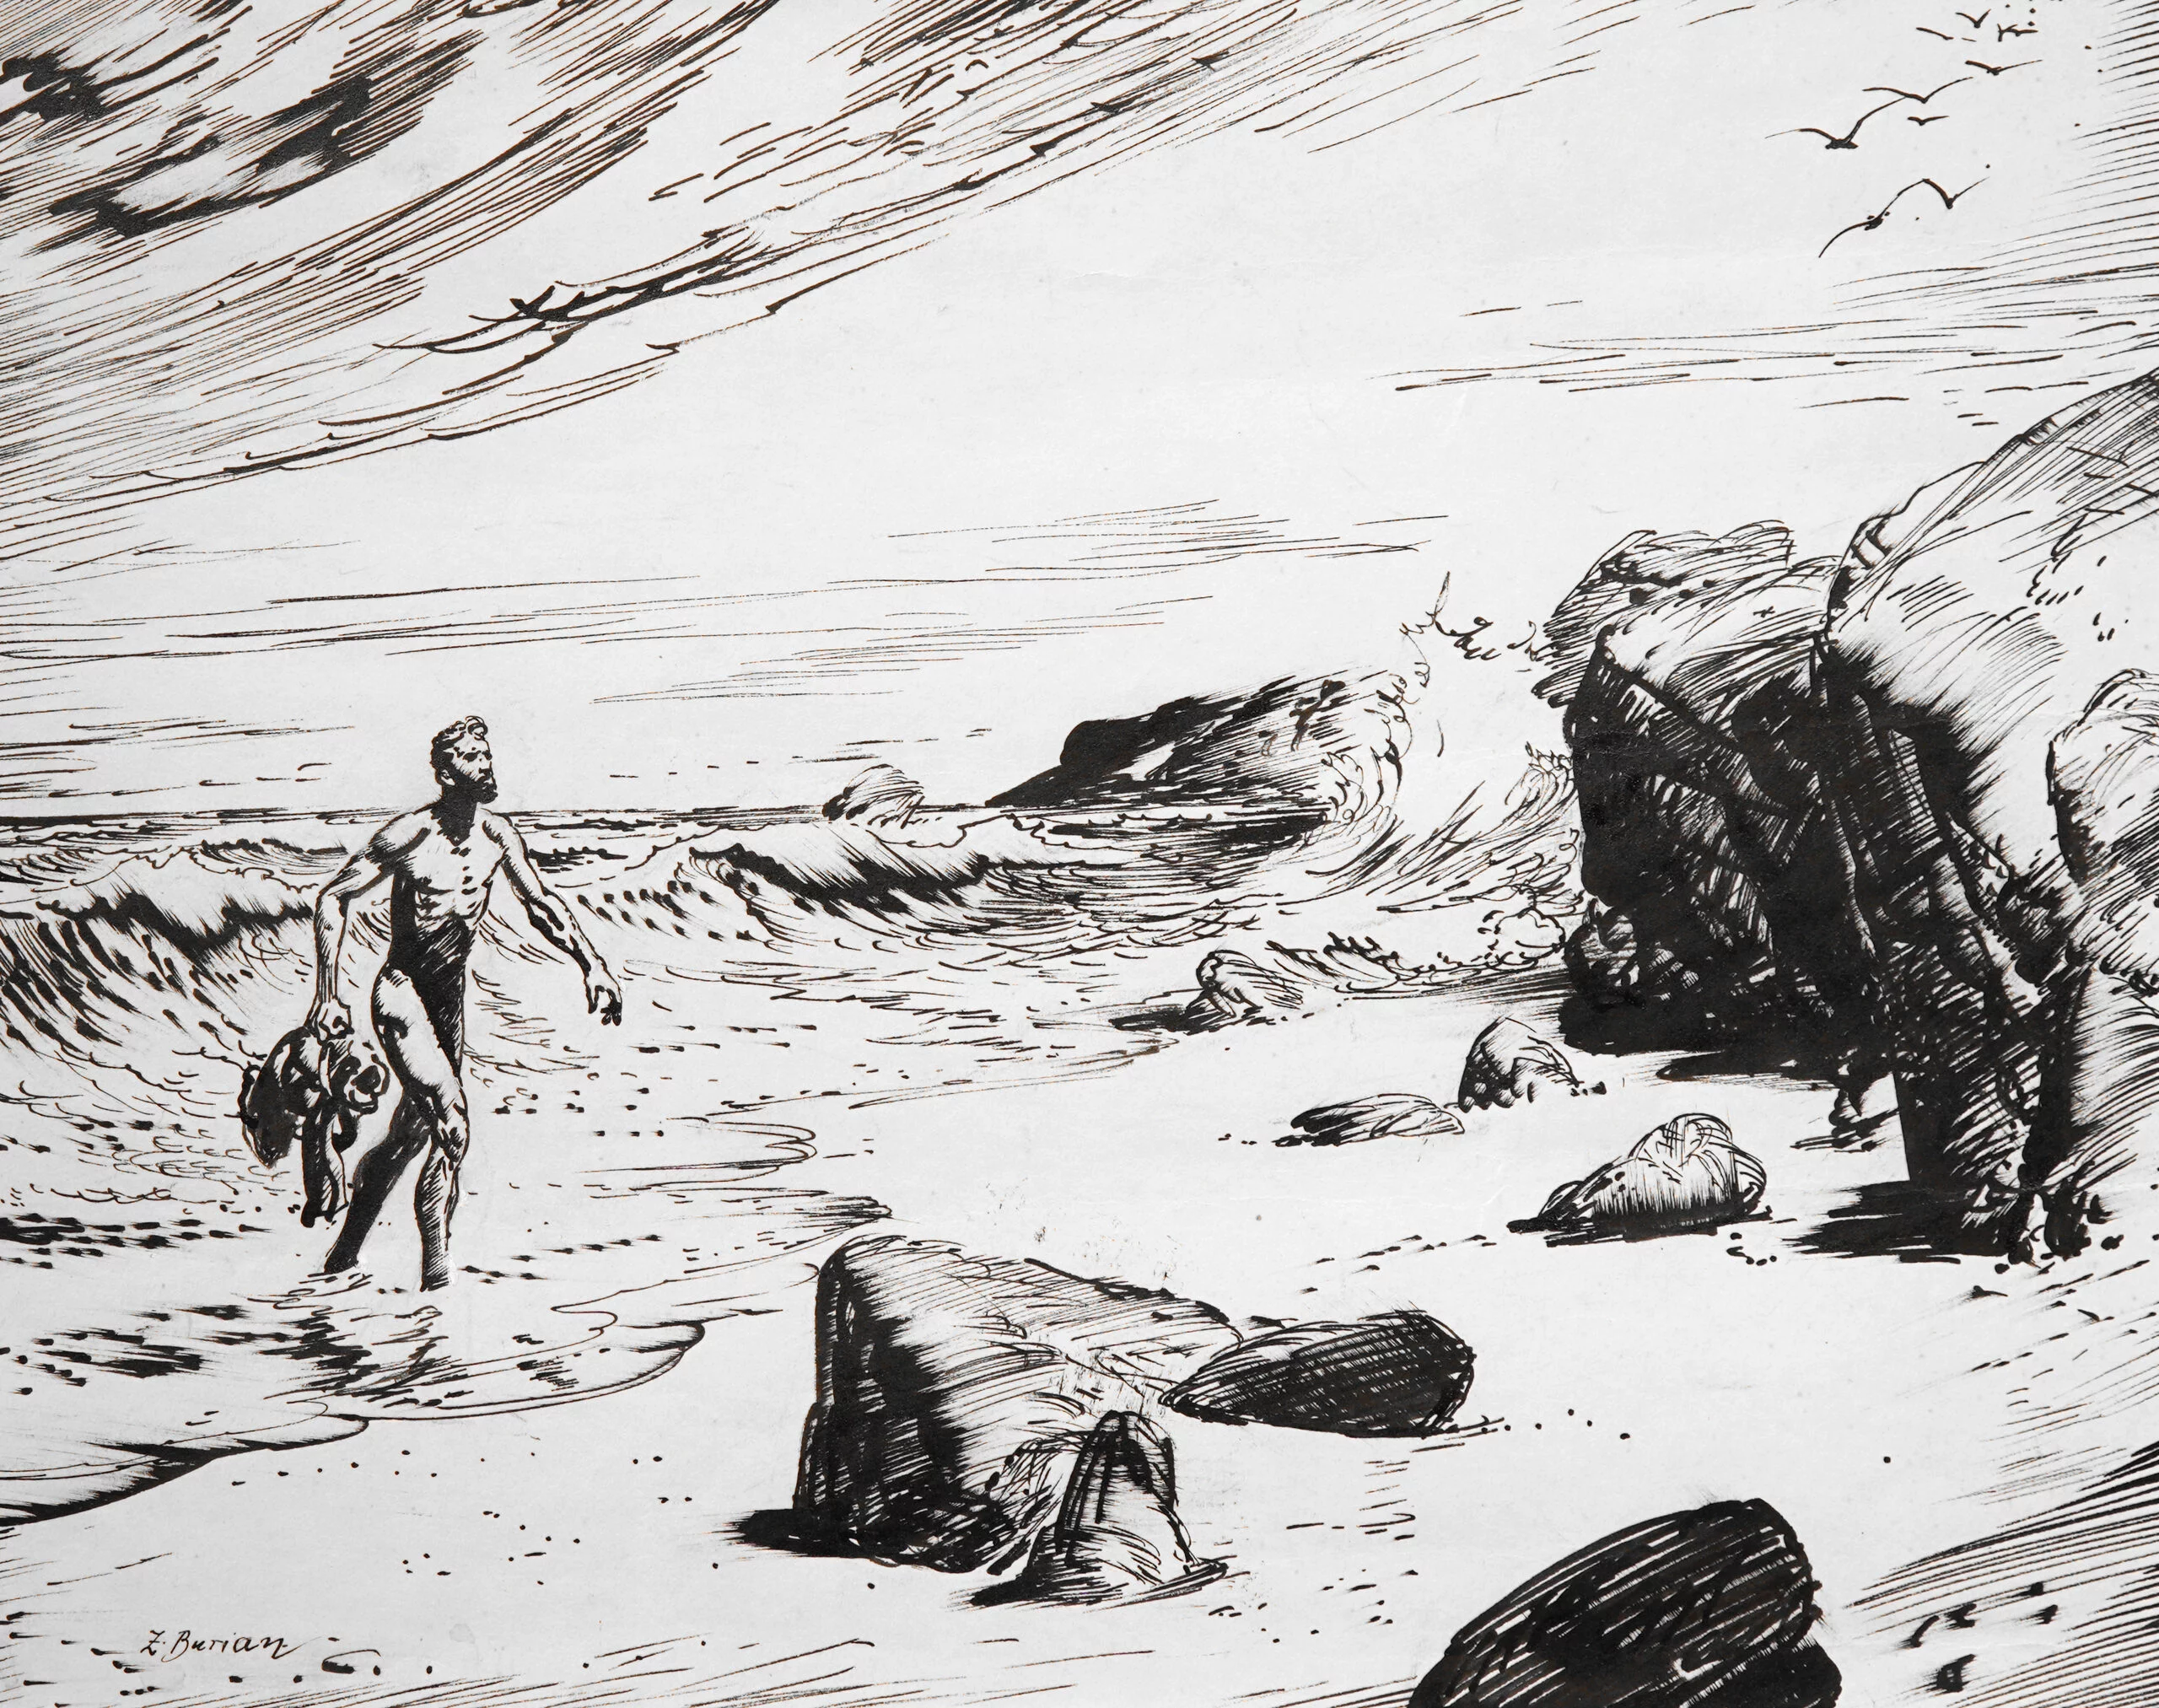
\includegraphics[width=0.95\textwidth]{jules}
	\caption{\href{https://aukceaukci.s3.amazonaws.com/aukceaukci/production/files/2024/02/06/10/15/12/906b839a-538e-4f31-bbcc-131d423cb646/1.webp}{source}}
\end{figure}

\begin{document}
\chapter{Aspekty a body osudu}
\label{chap:aspekty}

\section{Aspekty, narativ a příběhová pravomoc}
\label{sec:aspekty-narativ-pribeh}

``Pod vším ve Fate hledej aspekty''. Skutečně, aspekty hrají ve Fate Core zcela zásadní roli. Jsou tím, co je na těchto pravidlech typické a bez nich by Fate Core nebyl Fate Core.

\begin{itemize}
\item postavy, nejdůležitější součást hry, jsou definovány a vymezeny pomocí aspektů (\asp{Špinavý žoldák z Hlubiny, Hbitý skřítek z Imchejle, Čestný rytíř z řádu Devíti hvězd, Temperamemtní učednice Alwarina Bílého})
\item herní prostředí, tj. parkety, na kterých se odehrává drama postav, je nastaveno pomocí aspektů (\asp{Největší město na Taře, Prokleté údolí, Hora, kde sídlí bohové, Jeskyně plná drahokamů})
\item momentální stav prostředí, nálada scény, důležitý okamžitý detail jsou všechno věci vyjádřené pomocí aspektů (\asp{Podlaha v plamenech, Překážka v cestě, Tma jako v pytli, Něco tu sakra nehraje...})
\item významné předměty a vybavení jsou vytvářeny aspekty (\asp{Jiskřící čepel, Meč takzvaného Taranise, Kalich devítí duší, Havraní spár, Zaklínačské vybavení})
\item dovednosti se používají v akcích a akce zase jen upravují či těží z aspektů
\end{itemize}

\begin{sloppypar}
Výčet výše snad vyjasnil, že aspekty jsou podstatné. Co ale tedy takový aspekt je? Aby definice byla dostatečně obecná, ale nikoli zase vyprázdněná, je potřeba jí formulovat poněkud beztvaře: Aspekt je sousloví, fráze, věta, která popisuje jakoukoliv významnou vlastnost světa či významnou věc v onom světě. 
\end{sloppypar}

Pravidla aspektů unikátním způsobem kloubí vyprávění a mechanické hraní. Na jednu stranu, aspekty jsou deskriptivní - \emph{popisují}, jak scéna/místo vypadá, jaké postavy jsou; na stranu druhou je aspekty preskriptivní - \emph{stanovují}, jak scéna/místo \emph{odteď vypadá} (\asp{Všude to hoří, Po kolena ve vodě}) a jaké postavy \emph{odteď budou} (\asp{Trochu zkleslý, Zcela zmanipulovaný, Téměř mrtvý}). Tedy, mechanickým hraním lze svět kolem aktivně utvářet a spravovat, ne se jej pouze účastnit; cokoliv, co je aspektem, ve světě skutečně je a děje se. \\

Bývá zvykem, že většinu scén připravuje vypravěč, a tedy i aspekty scény. Nicméně, jakmile se hráči ve scéně objeví a začnou s aspekty interagovat, upravovat stávající a vytvářet nové, i narativ se podle toho mění - příběh vyprávějí oni. Tomu v těchto pravidlech říkáme, že všichni hráči mají \emph{vypravěčskou pravomoc}. Role vypravěčě je prostě reagovat na vyprávění ostatních hráčů - skrze nehráčské postavy (neboť např. zná jejich motivaci, cíle apod.) a skrze herní prostředí (zná, co je za těmito dveřmi, kam vede tato chodba a jak citlivá je past pod podlahou). Je ovšem zcela zásadní si uvědomit, že vyprávění příběhu je opravdu záležitostí (povinností) každého z družiny, nikoli pouze vypravěče. \sidenote{A taky je to zábavnější (a o to nám jde!). Vypravěč, byť jistě v dobré vůli, nedokáže připravit dobrodružství tak, aby se všem líbilo. Je proto na zodpovědnosti každého hráče, aby pomocí své vypravěčské pravomoci vytvořil příběh, který pro něj (jeho postavu) bude dokonalý.} \\

V další části textu detailně rozebereme, s jakými aspekty se lze potkat, co vyjadřují, jak je měnit či vytvářet. Ještě předtím je ale dobré rozebrat, jak vypadá dobrý aspekt.

\subsection{Jak vypadá dobrý aspekt}
\label{sec:jakvypadadobry}

Jak jsme měli možnost vidět, aspekty tvoří hru a hra tvoří aspekty. Nicméně, aby aspekt svoji roli plnil dobře, existuje několik zásad, jak jej formulovat. Později (v další sekci) uvidíme, že takto formulovaný aspekt se jednoduše vynucuje, tedy je pro nositele dobrým zdrojem bodů osudu (pokud je aspekt spojen s postavou). Pro jednoduchost jsou vlastnosti líčeny na příkladu aspektů postav.\\

Tak v první řadě, dobrý aspekt je \textbf{dvousečný} \sidenote{Ve skutečnosti žádná ``sečnost'' neexistuje, tj. neexistuje ``negativní a pozitivní'' aspekt. Aspekt je prostě věta, co sama o sobě nenese žádné hodnocení.}; říká, v čem se postava může blýsknout a v čem také může selhat. Díky tomu aspekt dobře slouží jak hráči, který jej nejspíše vyvolá, aby vysvětlil, jak mu v jeho počínání pomůže, tak stejně dobře poslouží vypravěči, aby upozornil, jak ho tento aspekt dostává do problémů. A v každém případě, dvousečně formulované aspekty jsou prostě zábavnější: \asp{Nikdo mě nikdy nemůže porazit} je munchkinovské, kdežto \asp{Říkám o sobě, že mě nikdy nikdo nemůže porazit} se může hezky zvrtnout. Podobně, aspekt \asp{Chodicí encyklopedie} neumožňuje žádné jiné použití než ukázka toho, jak inteligentní a sečtělá postava je. Na druhou stranu aspekt \asp{Podivínský milovník knih} lze kromě téhož účelu použít i v situaci, kdy se projeví, že postava většinu svého života strávila v knihovně...

Druhým důležitým specifikem dobrého aspektu je, že \textbf{říká více než jen jednu věc}. Zde začněme příkladem: aspekt \asp{Hledaný} je poměrně obecný, vlastně až přílíš. Je z něj patrná pouze jediná věc, totiž že postavu někdo hledá. Kdežto aspekt \asp{Hledá mě Noční let} specifikuje, že postavu hledá právě Noční let - a že se tedy vůči němu nějak provonil, má nějaké informace, apod. Najednou postava ožívá, má dimenzi navíc - se světem ji nyní spojuje vztah s Nočním letem. \sidenote{Zde by šlo navrhnout, že specifikací Nočního letu už není možné, aby postavu hledal někdo jiný, tj. hráč přichází o možnosti vynucení. To je ovšem na šikovnosti Vypravěče - vždy se přeci může stát, že Noční let si najme někoho dalšího, že jeho identitu prodá apod.}\\

Poslední vlastností, kterou zde uvedeme, je \textbf{jasná formulace}. Aspekt je nějaká věta psaná nedokonalým jazykem a konečným počtem slov. I tak by měl být ale formulován takovým způsobem, aby všichni měli představu, co znamená. V opačném případě jej nemohou správně použít. Příkladem budiž aspekt \asp{Vzpomínky na dětství} - je cítit, že vyvolává jistou nostalgii a že pro postavu bylo asi dětství podstatné při formování osobnosti. Ale \emph{jakým způsobem podstatné?} To z aspektu není zřejmé. Kdežto aspekty \asp{Dětství plné šikany, Vyrůstal jsem mezi šlechtou na zámku, Za všechno dlužím rodině} jasně dokreslují, o jaké dětství asi mohlo jít.\\

Pozorný čtenář nyní namítne, že v uvedených příkladech u každého ze specifik se ne vždy odrážejí i specifika ostatní. A to je pravda. Je vždy totiž podstatné brát kontext - pokud se hráči shodnou, že i neideálně formulovaný aspekt je pro ně dost dobrý (resp. si ho vždy dokáží přeformulovat ve své hlavě tak, aby byl dost dobrý), není důvod trávit hodiny vymýšlením chytrých frází, které by všechny požadavky odškrtly. Dost pravděpodobně by takto formulovaný aspekt působil uměle, slovosled by byl kostrbatý a věta strašně dlouhá.

\section{Body osudu a obnova}
\label{sec:body-osudu-obnova}

Vylíčili jsme, kde všude se lze s aspekty ve Fate setkat. Co jsme ovšem zatím nezmínili je, jakým způsobem aspekty zasahují do mechanického hraní. Stěžejní zde budou body osudu (tzv. fate points) coby platidlo, za které lze ``uplácet osud''. \\

Na začátku každého sezení začínají všichni hráči s tolika body osudu, kolik činí jejich obnova. V základu je to tři, nicméně každý hráč se může rozhodnout (při vytváření postavy a při určitých milnících) snížit svoji obnovu na úkor počtu triků. Za každou jednu ubranou obnovu si může napsat nový trik, nesmí ale s obnovou klesnout pod jedna.

Všehovšudy se bodů osudu a aspektů týkají 2 mechaniky: \textbf{vyvolání a vynucení aspektu}; první používá typicky hráč, aby si přilepšil, kdežto druhou nejčastěji používá vypravěč, aby hráčům život zkomplikoval (tedy ehm, vylepšil hru).

\subsection{Vyvolání aspektu}
\label{sec:vyvolani-aspektu}

Nejjednodušším způsobem, jak použít aspekt, je vyvolat jej. To lze několika způsoby, přičemž za každé použítí platí hráč jeden bod osudu. V případě, že hráč používá aspekt své postavy či aspekt scény, zaplacený bod osudu putuje do banku; v situaci ale, kdy používá aspekt jiné postavy (a tím jsou i následky!), zaplacený bod osudu jde do kapsy této postavy.\sidenote{Je zřejmé, že ve většině případů se nevyplatí příliš vyvolávat aspekty protivníku. Na druhou stranu, dost často se může stát, že žádné jiné zrovna nejsou relevantní - např. bojová postava se snaží zvítězit v sociálním konfliktu a nemá jiný způsob, než použít protivníkův aspekt \asp{Prý bije svoji ženu}; podobně např. nebojová postava ve fyzickém konfliktu.}

\begin{pravidlo}[Použití aspektu 1]
\begin{enumerate}
\item použít aspekt k vytvoření narativního detailu
\item použít aspekt ke změně výsledku hodu
\item použít aspekt k zvýšení pasivní opozice o +2 (nebo vytvoření pasivní opozice +2, pokud předtím opozice neexistovala)
\item použít aspekt a přidat bonus +2 k hodu jiné postavy
\end{enumerate}
\end{pravidlo}

První způsob se odkazuje na vypravěčskou pravomoc každého z hráčů a fakt, že existující aspekt hovoří o narativní skutečnosti. 

\begin{příklad}
Družina se ocitne ve městě s aspektem \asp{Ty ulice mají uši} a potřebuje zjistit nějaké informace o události, co se v ulicích nedávno stala. To lze dosáhnout mnoha způsoby, ideálně dovednostmi jako \dov{Kontakty, Vyšetřování} apod. Družina se nicméně z různých důvodů \sidenotemark  může rozhodnout pro jiné řešení: zaplatí bod osudu na vyvolání aspektu \asp{Ty ulice mají uši} aby zahlásili, že onen žebrák, se kterým se zrovna baví, na místě činu byl, a tudíž má informace, které oni potřebují (ale to, že je má, neznamená, že jim je jen tak vydá...).\\
\end{příklad}
\sidenotetext{Například žádný z hráčů v družině nemá dovednosti na dobré úrovni, či nechtějí riskovat neúspěch atd.}
Druhý způsob se využívá, když není postava spokojena s výsledkem svého hodu. Může popsat, jak jí nějaký aspekt umožňuje výsledek ještě zvrátit a

\begin{pravidlo}[Použití aspektu 2]
\begin{itemize}
\item buď si přidat +2 k výsledku hodu
\item nebo vzít všechny kostky a hodit ještě jednou
\end{itemize}
\end{pravidlo}

Zde je nutno podotknout, že takto nelze použít libovolný aspekt - musí dávat smysl, že ten onen je postavě zrovna schopen pomoci (ať už je to aspekt jeho postavy nebo např. scény). Samosebou, toto lze opakovat (má-li postava dost bodů osudu), platí nicméně, že k vylepšení výsledku téhož hodu není možné použít týž aspekt vícekrát.

Třetí způsob je trochu netradiční. Podobně jako první se opírá o vypravěčskou pravomoc, ale tentokrát jde skutečně o ``uplácení osudu''. Jen si to představte: zloděj před vašima očima krade váš poklad, přeskakuje propast a vrhá se na \asp{Žebřík ze shnilých provazů} - hod na \akc{Překonání} pomocí \dov{Mobility} s pastí +3. Vy propast nepřeskočíte, protože je moc široká, tak se na něj jen zamračíte, uplatíte osud a \emph{najednou se kus žebříku přetrhne} - a past je najednou +5... \sidenote{To se může zdát jako přespříliš silné. Narozdíl ale od aktivní opozice ale takto nikdy nelze přetočit kostky, není započten žádný váš bonus za dovednost a ani si nemůžete vybrat, na jakou budete házet. Samozřejmě, pokud se rozhodne 5 členů družiny vyšikanovat jednoho nepřítele, každý zaplatí bod osudu a přidá +2 (pokud existují unikátní aspekty, které lze vyvolat), tak má nepřítel problém. Na druhou stranu, tomu lze předcházet např. tím, že nepřítel má vlastní body osudu nebo předtím družinu dostatečně vyčerpal.}

Poslední způsob je vlastně podobný tomu třetímu, jen naopak. Typicky díky němu může družina na poslední chvíli pomoci nějaké postavě, které by jinak hrozila velká cena: nepřátelský zabiják se dostane k nic netušícímu čaroději a vypadá to, že čaroděj dočaroval... Jenže pak začnou padat body osudu, spoludružiníci použijí \asp{Zmapované bojiště, Improvizované krytí a Vítěznou vlnu} \sidenote{Všimnětě si, že nelze použít jeden aspekt třikrát.} a najednou má čaroděj k hodu bonus +6. \\

Jak vidno, body osudu jsou mocné platidlo a mohou zcela změnit vývoj hraní. Kromě obnovy existuje vlastně jediná mechaniky, jak body osudu získat - vynucování aspektů.

\subsection{Vynucování aspektů}
\label{sec:vynucovani-aspektu}

Aspekty, jakožto objektivní danost, slouží vypravěči (a vlastně nejen jemu), aby hráčům připomínal, že to, co jim dává výhodu, jim zároveň může i život komplikovat. Týž aspekt, který postava vyvolala ke svému prospěchu, může být použit k vynucení ``proti ní''.\\
Za každé vynucení, které hráč přijme, dostane jeden bod osudu. Může se však rozhodnout, že vynucení nepřijde - protože ale vychází z jeho daností, je nutné při svém popření uplatit osud a jeden bod osudu tak zaplatit. Vynucení typicky probíhá jedním ze dvou způsobů

\begin{enumerate}
\item vynucením rozhodnutí
\item vynucením události
\end{enumerate}

Vynucení rozhodnutí je aktuální vždy, když postava před nějakým rozhodnutím již stojí a kvůli (nejen svým) jistým aspektům je rozumné se domnívat, že se nějak konkrétně rozhodne. Například, postava s aspektem \asp{Nenávidím temné elfy} se dostane do situace, kde může prásknout svého pouštně-elfího spoludružiníka. Samozřejmě, to pro elfa nebude dobrá zpráva (a dost pravděpodobně ani pro práskače), ale s vynucením tohoto aspektu za to alespoň získá bod osudu...\\
Vynucení události se projeví spíše mimo scénu a nějakou tím započne. Příkladem budiž postava s aspektem \asp{Jdou po mně kněží Temné desítky} a návštěva Dunrileanu; i když se postava přímo nehrne do chudinské čtvrti mezi přisluhovače Sandol Kah, vynucením tohoto aspektu k tomuto setkání určitě dojde.
Z obou příkladů je zřejmé, že vynucení aspektu představuje pro postavu (či dokonce družinu) jistou komplikaci. Může se stát, že hráči nebudou chctít vynucení přijímat ze strachu, že situaci nebudou schopni vyřešit. Zde je důležité, aby vypravěč vždy na paměti měl smysl hraní - zábava. Neustálým předhazovaním nepřekonatelných výzev si nikdo nic neužije a hráče to nemotivuje vytvářet si postavy, které se do problému mohou dostávat. Ideální je, když panuje atmosféra, ve které hráči vypravěči věří, že jeho záměrem je skutečně dobrá hra a že vynucení je příležitost pro postavu získat aspekt. Zajímavým řešením je nechat hráče samotného vymyslet, jaké následky by pro něj komplikace mohla mít.
Stojí za poznamenání, že vynucení aspektů nemusí vždy provádět vypravěč jinému hráči. Ve skutečnosti vynutit může kdokoliv aspekt kohokoliv - platí ale, že bod osudu platí vynucovatel. %\sidenote{Vypravěč má pro vynucování nekonečný bank bodů osudu.}. 

\newpage{}
\end{document}

%%% Local Variables:
%%% mode: LaTeX
%%% TeX-master: "../main"
%%% End:
